\documentclass[11pt]{article}

\usepackage[letterpaper, margin=1in]{geometry}
\usepackage{listings}
\usepackage[spanish]{babel}
\usepackage[utf8]{inputenc}
\usepackage{multirow}
\usepackage{tabularx}
\usepackage{longtable}
\usepackage{graphicx}



%Figuras
\usepackage{graphicx, subfigure}
\usepackage[]{tikz}
\usepackage{pbox}

%Matemática
\usepackage{amsmath}
\usepackage{amssymb}

%Símbolos mate extra (alfabetos, etc.)
\usepackage{mathrsfs}


%Algoritmos
\usepackage{float}
\usepackage{algorithm}
\usepackage{algorithmicx}
\usepackage{algpseudocode}
\usepackage{listings}


\usepackage{color}
\usepackage{hyperref}

\usepackage{mdframed}
\usepackage{tcolorbox}
\usepackage{multicol}
\usepackage{booktabs}
\usepackage{tabulary}
\definecolor{darkblue}{rgb}{0 , 0.054 , 0.196}



\title{Reporte de Laboratorio 6}
\author{Emmanuel Bustos - B51296 \\ Dunia Barahona - B40806}
\begin{document}

\maketitle
\hrule
\hrule
\tableofcontents
\hspace{5mm}
\hrule
\hrule


\section{Introducción}
Este laboratorio consistió en la creación de una clase grafo, con sus métodos básicos.
\subsection{Objetivos}
\begin{itemize}
	\item Aprender a crear e implementar grafos.
	
\end{itemize}

\section{Diagramas de clase}

\begin{figure}[!ht]
	\caption{Diagrama UML de la clase mazo}
	\centering
	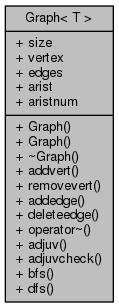
\includegraphics[width=0.16\textwidth]{1}
\end{figure}

\begin{figure}[!ht]
	\caption{Diagrama de dependencias}
	\centering
	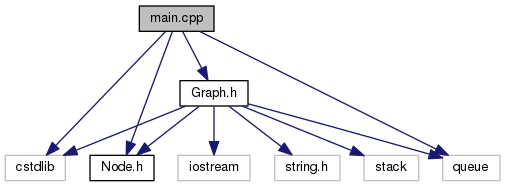
\includegraphics[width=1\textwidth]{2}
\end{figure}

\newpage

\section{Código}
\subsection{Clase Nodo (Vértice)}
\begin{lstlisting}


#ifndef NODE_H

#define NODE_H


template <typename T> class Node {

public:


T D;

///Constructor de la clase nodo

Node() {

};

///Constructor sobrecargado de la clase nodo

Node(Node* l, Node* r, Node* p, T* d) {

D = d;

};

///Destructor de la clase nodo

virtual ~Node() {

};


private:


};


#endif /* NODE_H */
\end{lstlisting}

\subsection{Clase Grafo}
\begin{lstlisting}

#ifndef GRAPH_H
#define GRAPH_H

#include "Node.h"
#include <iostream>
#include <cstdlib>
#include "string.h"
#include <queue>
#include <stack>
using namespace std;


template <typename T> class Graph {
public:
int size;
Node<T>* vertex;
bool** edges;
Node<T>** arist;
int aristnum;

///Constructor de la clase grafo
Graph() {
size=0;
aristnum=0;
vertex = 0x0;
edges = 0x0;
arist=0x0;
};

///Constructor sobrecargado de la clase grafo
Graph(int si, Node<T>* r) {
this->size = si;
this->vertex = r;
aristnum=0;
arist=0x0;
edges=0x0;
};

///Destructor de la clase grafo
virtual ~Graph() {
delete[] vertex;
for(int i=0;i<size;i++){
delete[] edges[i];
}
delete edges;
};

///Funcion que crea un vertice con tipo de dato generico
void addvert(Node<T> n){
Node<T>* vert=new Node<T>[this->size+1];
bool** edge = new bool*[size+1];
for(int i=0; i<size; i++){
edge[i] = new bool[size+1];
}
edge=this->edges;
for(int j=0;j<size+1;j++){edges[size+1][j]=false;}
for(int i=0; i<size;i++){
vert[i].D=vertex[i].D;
}
this->size=this->size+1;
vert[size-1]=n;
delete[] vertex;
this->edges=edge;
this->vertex=vert;
}

///Funcion que remueve un vertice
void removevert(int n){
Node<T>* vert=new Node<T>[this->size-1];
bool** edge = new bool*[size-1];
for(int i=0; i<size; i++){
edge[i] = new bool[size-1];
}
edge=this->edges;
int i=0;
int k=0;
while(i<size-1){
if(i==n){
k++;
}
int m=0;
for(int j=0;j<size;j++){
if(j==n){m++;}
edge[i][j]=this->edges[k][m];
m++;
}
vert[i].D=vertex[k].D;
i++;
k++;
}
this->size=this->size-1;
delete[] vertex;
this->edges=edge;
this->vertex=vert;
}

///Funcion que cra una arista
void addedge(int a, int b){
Node<T>** vert=new Node<T>*[this->aristnum+1];
for(int i=0; i<aristnum+1; i++){
vert[i] = new Node<T>[2];
}
for(int i=0; i<aristnum;i++){
vert[i][0].D=arist[i][0].D;
vert[i][1].D=arist[i][1].D;
}
this->aristnum=this->aristnum+1;
vert[aristnum-1][0]=vertex[a];
vert[aristnum-1][1]=vertex[b];
delete[] arist;
this->arist=vert;
this->edges[a][b]=true;
this->edges[b][a]=true;
}

///Funcion que elimina una arista
void deleteedge(int a, int b){
Node<T>** vert=new Node<T>*[this->aristnum-1];
for(int i=0; i<aristnum-1; i++){
vert[i] = new Node<T>[2];
}
int i=0;
int k=0;
while(i<aristnum-1){
if(arist[i][0].D==vertex[a].D && arist[i][1].D==vertex[b].D){
k++;
}

vert[i][0].D=arist[k][0].D;
vert[i][1].D=arist[k][1].D;
i++;
k++;
}
this->aristnum=this->aristnum-1;
delete[] arist;
this->arist=vert;
this->edges[a][b]=false;
this->edges[b][a]=false;
}

///Funcion que imprime los datos del grafo
void operator~(){
cout<<"Vertices: "<<endl;
cout<<"(";
for(int i =0; i<size-1;i++){
cout<<vertex[i].D<<", ";
}
cout<<vertex[size-1].D<<")"	;
cout<<endl;
cout<<"Aristas:"<<endl;
cout<<"(";
for(int i =0; i<aristnum-1;i++){
cout<<"(";
cout<<arist[i][0].D<<", ";
cout<<arist[i][1].D<<"), ";
}
cout<<"(";
if(aristnum!=0){
cout<<this->arist[aristnum-1][0].D<<", ";
cout<<arist[aristnum-1][1].D<<"))";
}
cout<<endl;
cout<<"Adyacencia: "<<endl;
cout<<"  ";
for(int i =0; i<size;i++){
cout<<vertex[i].D<<" ";
}
cout<<endl;
for(int i =0; i<size;i++){
cout<<vertex[i].D<<" ";
for(int j =0; j<size;j++){
if(this->edges[i][j]==false){cout<<"F ";}
else if(this->edges[i][j]==true){cout<<"T ";}
}
cout<<endl;
}
}

///Funcion que retorna los vertices adjuntos a un vertice especifico dado
int adjuv(int n, bool* visvec){
visvec[n]=true;
int find=size;
int i=0;
while(find>0){
if(edges[n][i]==true && visvec[i]==false){
visvec[i]=true;
return i;
}
find--;
i++;
if(find==0){//cout<<"No hay mas vertices adyacentes"<<endl; 
return 0;}
}

}

///Funcion que verifica si un vertice posee vertices adjuntos
int adjuvcheck(int n, bool* visvec){
int find=size;
int i=0;
while(find>0){
if(edges[n][i]==true && visvec[i]==false){
return i;
}
find--;
i++;
if(find==0){//cout<<"No hay mas vertices adyacentes"<<endl; 
return 0;}
}

}
///Funcion que imprime el camino a seguir ara una busqueda por ancho
void bfs(){
bool* visvec = new bool[size];
queue<int> cola;
int* camino=new int[size];
int pos=0;
int m=0;
for(int i=0; i<size; i++){
visvec[i]=false;
}
visvec[0]=true;
int i =0;
camino[i]=0;
i++;
int estado=3;
while(adjuvcheck(pos,visvec)!=0){
camino[i]=adjuv(pos,visvec);
cola.push(camino[i]);
estado=camino[i];
i++;
}
pos=cola.front();
cola.pop();
bool busqueda =true;
while(busqueda){
if(cola.size()==0){busqueda=false;}
while(adjuvcheck(pos,visvec)!=0){
camino[i]=adjuv(pos,visvec);
cola.push(camino[i]);
i++;
}
pos=cola.front();
cola.pop();
}
cout<<"El recorrido por ancho es: ("; for(int j=0; j<i-1;j++){cout<<camino[j]<<", ";} cout<<camino[i-1]<<")"<<endl;
cout<<"(Valores: ("; for(int j=0; j<i-1;j++){cout<<vertex[camino[j]].D<<", ";} cout<<vertex[camino[i-1]].D<<"))"<<endl;
}
///Funcion que ejecuta una busqueda de profundidad en el grafo
void dfs(){
bool* visvec = new bool[size];
stack<int> stack;
int* camino=new int[size];
int pos=0;
for(int i=0; i<size; i++){
visvec[i]=false;
}
visvec[0]=true;
int i =0;
camino[i]=0;
stack.push(pos);
i++;
while(stack.size()!=0){
if(adjuvcheck(pos,visvec)!=0){
camino[i]=adjuv(pos,visvec);
stack.push(camino[i]);
pos=camino[i];
i++;
}
if(adjuvcheck(pos,visvec)==0){
pos=stack.top();
stack.pop();
}
if(pos==0){
camino[i]=adjuv(pos,visvec);
stack.push(camino[i]);
pos=camino[i];
i++;
}
}
cout<<"El recorrido por profundad es: ("; for(int j=0; j<i-1;j++){cout<<camino[j]<<", ";} cout<<camino[i-1]<<")"<<endl;
cout<<"(Valores: ("; for(int j=0; j<i-1;j++){cout<<vertex[camino[j]].D<<", ";} cout<<vertex[camino[i-1]].D<<"))"<<endl;
}
private:

};

#endif /* Graph_H */

\end{lstlisting}


\subsection{Main}
\begin{lstlisting}
#include <cstdlib>
#include "Node.h"
#include "Graph.h"
#include <queue>
#define NL cout << endl;
#define SP " "

using namespace std;

int main(int argc, char** argv) {

int size=10;
Node<int> _1;
_1.D=1;
Node<int> _2;
_2.D=2;
Node<int> _3;
_3.D=3;
Node<int> _4;
_4.D=4;
Node<int> _5;
_5.D=5;
Node<int> _6;
_6.D=6;
Node<int> _7;
_7.D=7;
Node<int> _9;
_9.D=9;
Node<int> _10;
_10.D=10;
Node<int> _11;
_11.D=11;
Node<int>* vert=new Node<int>[1];
bool** edges = new bool*[size+1];
for(int i=0; i<size; i++){
edges[i] = new bool[size+1];
}
edges[0][0]=false;
vert[0]=_1;
Graph<int>* T = new Graph<int>();
T->vertex=vert;
T->size=1;
T->edges=edges;
T->addvert(_5);
T->addvert(_7);
T->addvert(_1);
T->addvert(_4);
T->addvert(_6);
T->addedge(2,3);
T->addedge(4,0);
T->addedge(0,2);
T->addedge(2,3);
T->addedge(4,5);
T->addedge(1,3);
~*T;
queue<int> cola;
cola.push(2);
cola.push(5);
cola.pop();
bool* g = new bool[4];
g[0]=true;
g[1]=false;
g[2]=false;
g[3]=false;
//cout<<T->adjuv(3, g)<<endl;
//cout<<T->adjuv(0, g)<<endl;
T->dfs();
T->bfs();
//cout<<T->arist[1][1].D<<endl;
return 0;
}

\end{lstlisting}

\section{Conclusiones}
Este laboratorio dotó al estudiante de las habilidades necesarias para comprender, crear e implementar las estructuras de datos abstractos grafos, así como la utilización de sus métodos básicos.




\end{document}
